\begin{figure}[t]
\centering
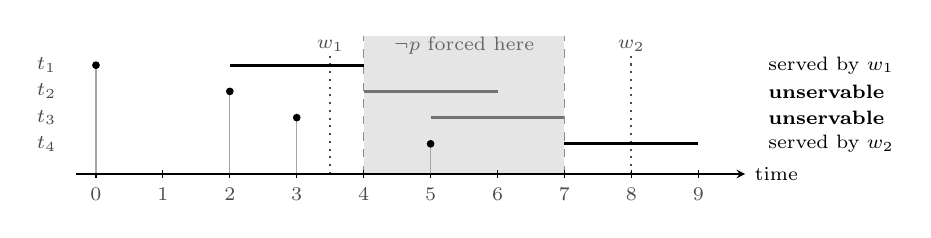
\begin{tikzpicture}[x=8.5mm,y=3.33mm,font=\scriptsize,>=stealth]

% band where p is forbidden
\fill[black!10] (4,-0.75) rectangle (7,4.5);
\draw[black!45,dashed] (4,-0.75) -- (4,4.5);
\draw[black!45,dashed] (7,-0.75) -- (7,4.5);
\node[black!60] at (5.5,4.15) {$\lnot p$ forced here};

% candidate times for p
\draw[black!70,dotted,thick] (3.5,-0.75) -- (3.5,3.9);
\node[black!70] at (3.5,4.15) {$w_1$};
\draw[black!70,dotted,thick] (8,-0.75) -- (8,3.9);
\node[black!70] at (8,4.15) {$w_2$};

% time axis
\draw[->] (-0.3,-0.75) -- (9.7,-0.75) node[right] {time};
\foreach \t in {0,1,2,3,4,5,6,7,8,9}
  \draw (\t,-0.9) -- (\t,-0.6) node[below=3pt,black!70] {$\t$};

% onset marks, named on the left
\foreach \o/\r/\lab in {0/3.4/{$t_1$}, 2/2.4/{$t_2$}, 3/1.4/{$t_3$}, 5/0.4/{$t_4$}} {
  \node[anchor=east,black!70] at (-0.45,\r) {\lab};
  \draw[black!35] (\o,\r) -- (\o,-0.7);
  \fill (\o,\r) circle (1.4pt);
}
% windows [t_i+2, t_i+4]
\draw[very thick] (2,3.4) -- (4,3.4);
\draw[very thick,black!55] (4,2.4) -- (6,2.4);
\draw[very thick,black!55] (5,1.4) -- (7,1.4);
\draw[very thick] (7,0.4) -- (9,0.4);

\node[anchor=west] at (9.9,3.4) {served by $w_1$};
\node[anchor=west] at (9.9,2.4) {\textbf{unservable}};
\node[anchor=west] at (9.9,1.4) {\textbf{unservable}};
\node[anchor=west] at (9.9,0.4) {served by $w_2$};

\end{tikzpicture}
\caption{The formula $\mathrm{AG}\,\mathrm{EF}_{[2,4]}\,p\wedge\mathrm{AG}_{[4,7]}\lnot p$ (\UNSAT). The bar at
$t_i$ is that onset's window $[t_i+2,t_i+4]$, and a $p$ at $w$ serves the onsets whose bar contains
it. The pursuit launched at $t_1$ stops at $w_1$ and serves no later onset.}\label{fig:onsets}
\end{figure}
